\chapter*{Capítulo 3 \vspace{0.5cm} \break Validación del nuevo sistema de capacitación}
\setcounter{chapter}{3}
\setcounter{section}{0}
\addcontentsline{toc}{chapter}{Capítulo 3: Validación del nuevo sistema de capacitación}

Partiendo del objetivo principal de esta investigación, rectificar las limitaciones existentes en el sistema SECPROIT, se desarrollaron un conjunto de pruebas y experimentos para demostrar que se enmendaron dichas restricciones. En el siguiente capítulo se presentan los resultados obtenidos en cada una de las pruebas. Este proceso parte de cómo la fase de análisis y diseño se unen para llevar a cabo el sistema propuesto.

\section{Pruebas funcionales}
 Las pruebas de software, o pruebas funcionales, son el proceso de ejecutar un sistema o componente para medir su calidad, con la intención de encontrar errores que aún no se descubren \cite{Buehler2008}.

Para este software, el nivel de prueba que se utiliza es: pruebas de sistema. Consiste en ejecutar el sistema completo, buscando defectos tanto en aspectos generales como en particulares. Se utilizan pruebas basadas en las funcionalidades (pruebas funcionales) y el método que se emplea es el de caja negra (se lleva a cabo sobre la interfaz del software) \cite{Nidhra2012}.

\subsection{Casos de prueba para la configuración entrenamientos}
Como se pudo apreciar en el capítulo 2, en el sistema desarrollado se introdujeron nuevas entidades, entre ellas: la configuración de un entrenamiento. Con esta configuración el jefe de área puede decidir el tiempo que puede tomar completar el entrenamiento de una etapa, el tipo de preguntas que pueden aparecer, la cantidad de intentos totales permitidos por cada etapa y la cantidad de intentos aprobados necesarios para superar cada una.

Gracias a esta nueva configuración, se lograron resolver algunas de las limitaciones que se mencionaban en el capítulo 1: 
\begin{itemize}
\item Existe más de un modelo de pregunta, solucionando el problema de escasez en el método de aprendizaje
\item Las etapas no aparecen de forma continúa, porque para poder avanzar a la siguiente se debe aprobar la etapa actual un número determinado de veces
\item Solo aparece una etapa a la vez
\item Para cada etapa existe más de un entrenamiento
\end{itemize}

Sin embargo, es necesario probar el correcto funcionamiento de este nueva entidad. Con ese fin, se diseñaron tres casos de prueba  (\textsl{Tabla \ref{cas1}}, \textsl{Tabla \ref{cas2}}, \textsl{Tabla \ref{cas3}}), cada una con sus propios experimentos. 

\subsubsection{Casos de prueba: Insertar configuración de entrenamiento}
El proceso de crear una nueva configuración de entrenamiento se realiza al insertar un nuevo proceso (todo ocurre en la misma interfaz de usuario). Para este caso de prueba se realizaron tres experimentos:

\begin{table}[H]
\begin{center}
\begin{tabular}{ | p{4cm} | p{3.8cm} | p{3.1cm} | p{3.2cm} |}
\hline
\centering\textbf{Prueba} & \textbf{Descripción} & \textbf{Resultado \break esperado} & \textbf{Resultado \break obtenido} \\
\hline
Insertar configuración con campos en blanco & Una configuración de entrenamiento no puede contener información vacía & Los campos están llenos por defecto y la interfaz no debe permitir que se vacíen los campos & La interfaz no permitió que los campos fueran vaciados (Anexo \ref{fig:cb}) \\
\hline
Insertar configuración con campos incorrectos & La única forma de introducir información incorrecta es insertando un número de intentos verídicos mayor que el número de intentos total & Debe aparecer un mensaje de error & Aparece un mensaje de error (Anexo \ref{fig:ci}) \\
\hline
Insertar configuración con campos correctos & Introducir campos correctos & Se debe introducir la configuración  & Se introdujo la nueva configuración (Anexo \ref{fig:cc}) \\
\hline
\end{tabular}
\caption{Casos de prueba: Insertar configuración de entrenamiento}
\label{cas1}
\end{center}
\end{table}

\subsubsection{Casos de prueba: Modificar configuración de entrenamiento}
El proceso de modificar la configuración de un entrenamiento se realiza al modificar un proceso (todo ocurre en la misma interfaz). Para este caso de prueba se realizaron tres experimentos:

\begin{table}[H]
\begin{center}
\begin{tabular}{ | p{4cm} | p{4cm} | p{3.1cm} | p{3cm} |}
\hline
\centering\textbf{Prueba} & \textbf{Descripción} & \textbf{Resultado \break esperado} & \textbf{Resultado \break obtenido} \\
\hline
Modificar configuración con campos en blanco & Una configuración de entrenamiento no puede contener información vacía & Los campos están llenos por defecto y la interfaz no debe permitir que se vacíen los campos & La interfaz no permitió que los campos fueran vaciados \\
\hline
Modificar configuración con campos incorrectos & La única forma de introducir información incorrecta es insertando un número de intentos verídicos mayor que el número de intentos total & Debe aparecer un mensaje de error & Aparece un mensaje de error \\
\hline
Modificar configuración con campos correctos & Introducir campos correctos & Se debe modificar la configuración  & Se modificó la configuración \\
\hline
\end{tabular}
\caption{Casos de prueba: Modificar configuración de entrenamiento}
\label{cas2}
\end{center}
\end{table}

\subsubsection{Casos de prueba: Eliminar configuración de entrenamiento}
Como medida de seguridad en el nuevo sistema de capacitación, el proceso de eliminar la configuración de un entrenamiento no existe de manera visual. Para eliminarla, debe eliminarse el proceso al que esta pertenece. Por lo tanto, el único experimento que se puede realizar en este caso es: eliminar un proceso.

\begin{table}[H]
\begin{center}
\begin{tabular}{ | p{2.7cm} | p{5.2cm} | p{3.1cm} | p{3.2cm} |}
\hline
\centering\textbf{Prueba} & \textbf{Descripción} & \textbf{Resultado \break esperado} & \textbf{Resultado \break obtenido} \\
\hline
Eliminar proceso & Se selecciona de una tabla el proceso que se desea eliminar & Se debe eliminar el proceso & Se eliminó el proceso (Anexo \ref{fig:ce}) \\
\hline
\end{tabular}
\caption{Casos de prueba: Eliminar configuración de entrenamiento}
\label{cas3}
\end{center}
\end{table}

\subsection{Casos de prueba para el entrenamiento en la etapa de las causas}
En el sistema SECPROIT, la etapa de las causas no se evalúa correctamente. Si la variable presenta más de una causa, el sistema evalúa la primera pero no logra evaluar las demás. En cambio, si del grupo de variables solo una se encuentra fuera de rango, la etapa de las causas no se evalúa en absoluto.

Sin embargo, el nuevo sistema desarrollado no presenta esta dificultad. En el software, para cada tipo de pregunta en la etapa de las causas, se evalúan un número distinto de variables (todas fuera de rango). Por ejemplo, en las preguntas de completar los espacios en blanco se evalúan cinco variables distintas (todas fuera de rango) y de cada una se preguntan sus causas (Anexo \ref{fig:pregcaus}}), mientras que en las preguntas de enlazar, solo se pregunta por una variable, pero esta posee múltiples causas.

Para probar el correcto funcionamiento del entrenamiento en la etapa de las causas, se evaluaron cuatro entrenamientos de esta etapa (\textsl{Tabla \ref{cas:causa}}), uno por cada pregunta (verdadero o falso, completar los espacios en blanco, selección múltiple y enlazar). Como las preguntas que se generan en los entrenamientos son aleatorias, para estos casos de prueba el valor de datos de entrada no es relevante. Para afirmar que las respuestas son correctas, se establece una comparación entre las respuestas dadas por el sistema y las respuestas que brinda el motor de reglas (\textsl{JDrools}).

\begin{table}[H]
\begin{center}
\begin{tabular}{ | p{3cm} | p{5.9cm} | p{2.6cm} | p{2.6cm} |}
\hline
\centering\textbf{Prueba} & \textbf{Descripción} & \textbf{Resultado del JDrools} & \textbf{Resultado del sistema} \\
\hline
Verdadero o \break falso & Se presentan 5 variables con sus causas y se debe indicar si la afirmación es verdadera o falsa & Se acertaron 2 afirmaciones &  Se acertaron 2 afirmaciones \\
\hline
Completar los espacios en blanco & Se presentan 5 variables y de 1 a 5 causas, y se debe rellenar el espacio en blanco de manera que quede una expresión verdadera & Se acertaron 3 expresiones &  Se acertaron 3 expresiones \\
\hline
Enlazar & Se presenta 1 variable y 5 causas, y se deben enlazar las que correspondan a esa variable & Se acertaron 4 &  Se acertaron 4 \\
\hline
Selección múltiple & Se presenta 1 variable y 5 causas, y se deben seleccionar las que correspondan a esa variable & Se acertó 1 selección &  Se acertó 1 selección \\
\hline
\end{tabular}
\caption{Casos de prueba para el entrenamiento en la etapa de las causas}
\label{cas:causa}
\end{center}
\end{table}

\subsection{Casos de prueba para el entrenamiento en la etapa de las recomendaciones}
En el sistema SECPROIT, la etapa de las recomendaciones no se evalúa. Al concluir la evaluación de la etapa de las causas, el sistema califica la etapa de las recomendaciones de excelente y se acaba el entrenamiento (Anexo \ref{fig:errorRec}).

Sin embargo, en el nuevo sistema desarrollado si se evalúan las recomendaciones. Para cada tipo de pregunta se evalúan un número distinto de recomendaciones. Por ejemplo, en las preguntas de verdadero o falso se evalúan cinco recomendaciones, mientras que en las preguntas de enlazar, se evalúan de una a cinco.

Para probar el correcto funcionamiento del entrenamiento en la etapa de las recomendaciones, se evaluaron cuatro entrenamientos de esta etapa (\textsl{Tabla \ref{cas:reco}}), uno por cada pregunta. Como las preguntas que se generan en los entrenamientos son aleatorias, para estos casos de prueba el valor de datos de entrada no es relevante. Para afirmar que las respuestas son correctas, se establece una comparación entre las respuestas dadas por el sistema y las respuestas que brinda el motor de reglas (\textsl{JDrools}).

\begin{table}[H]
\begin{center}
\begin{tabular}{ | p{2.7cm} | p{6.2cm} | p{2.6cm} | p{2.6cm} |}
\hline
\centering\textbf{Prueba} & \textbf{Descripción} & \textbf{Resultado del JDrools} & \textbf{Resultado del sistema} \\
\hline
Verdadero o \break falso & Se presentan 5 causas con sus recomendaciones y se debe indicar si la afirmación es verdadera o falsa & Se acertó 1 afirmación &  Se acertó 1 afirmación \\
\hline
Completar los espacios en blanco & Se presentan 5 causas y de 1 a 5 recomendaciones, y se debe rellenar el espacio en blanco de manera que quede una expresión verdadera & Se acertaron 3 expresiones &  Se acertaron 3 expresiones \\
\hline
Enlazar & Se presenta 1 causa y 5 recomendaciones, y se deben enlazar las que correspondan a esa causa & Se acertaron 2 &  Se acertaron 2 \\
\hline
Selección múltiple & Se presentan 1 causa y 5 recomendaciones, y se deben seleccionar las que correspondan a esa causa & Se acertaron 2 selecciones &  Se acertaron 2 selecciones \\
\hline
\end{tabular}
\caption{Casos de prueba para el entrenamiento en la etapa de las recomendaciones}
\label{cas:reco}
\end{center}
\end{table}

\section{Pruebas de rango con signos}
Las pruebas de rangos con signo de Wilcoxon permiten comparar poblaciones cuando sus distribuciones no siguen una distribución normal (muestran asimetría) o cuando tienen un tamaño demasiado reducido para poder determinar si realmente proceden de poblaciones normales. Se utilizan para comparar el rango medio de dos muestras relacionadas y determinar si existen diferencias entre ellas \cite{Turcios2015}.

\subsection{Proceso de entrenamiento}
En el sistema SECPROIT, para generar un entrenamiento, se extraen y se leen los ficheros del proceso al que pertenece, almacenados en la base de datos. A partir de la información extraída, se generan las preguntas del entrenamiento. Para calificar las pruebas, se vuelven a extraer los ficheros de la base de datos y se vuelve a leer la información escrita en ellos. Realizar el proceso de esta forma, genera una demora extra en la ejecución del software.

En el nuevo sistema de capacitación, se decidió almacenar la información de los ficheros de los procesos, en nuevas tablas incorporadas en la base de datos (como ya se comentó en capítulos anteriores). Cuando se va a generar un entrenamiento, se extrae la información necesaria de las tablas, y se generan las preguntas. A la hora de evaluar el entrenamiento, se utiliza la misma información extraída anteriormente. Realizar el proceso de esta manera reduce el tiempo de ejecución del mismo.

Para probar que el tiempo de ejecución del proceso de entrenamiento es menor en el nuevo sistema de capacitación desarrollado, se utilizaron las pruebas de rango con signo de Wilcoxon \cite{Turcios2015}. Cabe señalar que:

\begin{itemize}
\item Ambos sistemas se ejecutaron en la misma máquina, con las mismas características
\item Cuando se realizaron las pruebas, solo se ejecutaba el sistema evaluado (no existía ningún otro proceso ejecutándose)
\item Ambas pruebas fueron cronometradas dentro del propio sistema para evitar errores humanos
\item Los ficheros de los procesos utilizados para las pruebas, son los mismos en ambos sistemas
\end{itemize}

Con esta prueba, se desea conocer la efectividad del método implementado en el nuevo sistema de capacitación para la lectura de la información de los ficheros de un nuevo entrenamiento, y para ello se toma una muestra aleatoria de 10 procesos del sistema de capacitación. Se registró el tiempo que demoró generar y evaluar un entrenamiento en el sistema SECPROIT y el tiempo que demoró en el nuevo sistema de capacitación. El tiempo se encuentra registrado en minutos. Los datos obtenidos se pueden observar en la Tabla \ref{pruebasConSigno}.

\begin{table}[H]
\begin{center}
\begin{tabular}{ | c | c | c | }
\hline
\centering & \textbf{Sistema SECPROIT} & \textbf{Nuevo sistema de capacitación} \\
\centering & \textbf{(tiempo en minutos)} & \textbf{(tiempo en minutos)} \\
\hline
 Proceso #1 & 5:09 & 0:51 \\
\hline
 Proceso #2 & 5:23 & 0:55 \\
\hline
 Proceso #3 & 6:15 & 1:05 \\
\hline
 Proceso #4 & 6:01 & 1:00 \\
\hline
 Proceso #5 & 5:09 & 0:50 \\
\hline
 Proceso #6 & 5:15 & 0:52 \\
\hline
 Proceso #7 & 5:29 & 0:56 \\
\hline
 Proceso #8 & 5:23 & 0:54 \\
\hline
 Proceso #9 & 4:09 & 0:33 \\
\hline
 Proceso #10 & 5:21 & 0:50 \\
\hline
\end{tabular}
\caption{Comparando el tiempo demorado en el entrenamiento de un proceso}
\label{pruebasConSigno}
\end{center}
\end{table}

Las hipótesis de esta prueba son: no hay diferencia en el proceso de entrenamiento entre un sistema y otro (\textbf{H}0), y el proceso de entrenamiento del nuevo sistema se ejecuta más rápido que el del sistema SECPROIT (\textbf{H}1). Se procede a calcular la solución de la prueba utilizando la herramienta R, para la función \textsl{wilcox.test()}. El resultado obtenido es el siguiente (\textsl{Figura \ref{fig:herrR}}):

\begin{figure}[H]
\centering
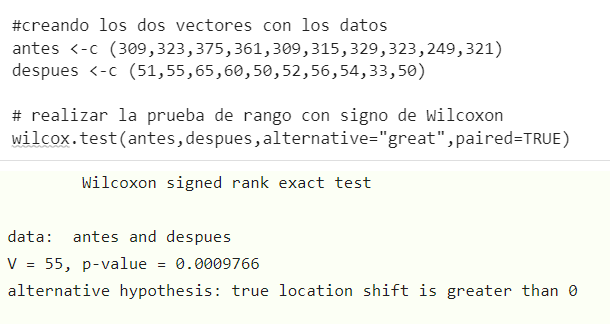
\includegraphics[width=0.9\linewidth]{imagen/erre.png}
 \caption{Resultados con la herramienta R}
 \label{fig:herrR} 
\end{figure}

El estadístico de prueba es 100 y el valor \textbf{p} correspondiente es 0.0001796. Dado que este valor \textbf{p} es menor que 0.05, se rechaza la hipótesis nula (\textbf{H}0). Existe una diferencia estadísticamente significativa entre el tiempo demorado en el sistema SECPROIT y el tiempo demorado en el nuevo sistema de capacitación. Por lo tanto, se puede afirmar que el nuevo método incorporado es mejor que el método anterior utilizado.

\section{Conclusiones parciales}
Al concluir este capítulo se pueden arribar las siguientes conclusiones:
\begin{itemize}
\item Se logró resolver la limitación existente en el proceso de entrenamiento de la etapa de las causas
\item Se logró resolver la limitación existente en el proceso de entrenamiento de la etapa de las recomendaciones
\item Se agregaron configuraciones al entrenamiento que permiten un mejor control de los mismos y una mejor evaluación
\item Se implementó un nuevo método para extraer la información de los ficheros de los procesos que resulta más rápido que el método anterior
\end{itemize}